
\documentclass[12pt]{article}
\usepackage[utf8]{inputenc}
\usepackage[a4paper]{geometry}
\usepackage{fancyhdr}
\usepackage{lastpage}
\usepackage{graphicx, wrapfig, subcaption, setspace, booktabs}
\usepackage[T1]{fontenc}
\usepackage[font=small, labelfont=bf]{caption}
\usepackage{fourier}
\usepackage[protrusion=true, expansion=true]{microtype}
\usepackage[english]{babel}
\usepackage{sectsty}
\usepackage{graphicx}
\usepackage{url, lipsum}
\usepackage{tgbonum}
\usepackage{hyperref}
\usepackage{pgfplots}
\usetikzlibrary{calc}
\usepackage{amsmath}
\usepackage{xcolor}
\usepackage[nottoc]{tocbibind} 
\usepackage{tikz}
\newcommand*\circled[1]{\tikz[baseline=(char.base)]{\node[shape=circle,draw,inner sep=2pt] (char) {#1};}}

%Adds "References" to the table of contents
\title{Bibliography management:\\\texttt{thebibliography} environment}


\newcommand{\HRule}[1]{\rule{\linewidth}{#1}}
\onehalfspacing
\setcounter{tocdepth}{5}
\setcounter{secnumdepth}{5}

\begin{document}
% Cover page
{\fontfamily{cmr}\selectfont
\title{ \normalsize \textsc{}
		\\ [2.0cm]
		\HRule{0.5pt} \\
		\LARGE \textbf{\uppercase{SOEN 6011 PROJECT DELIVERY ONE CALCULATOR OF FUNCTION 3(CF3) APPLICATION}
		\HRule{2pt} \\ [0.5cm]
		\normalsize \today \vspace*{5\baselineskip}}
		}
\date{}

\author{
		Xueying Li 40036265\\ 
		}

\maketitle

% Content
\newpage

\begin{normalsize}
        
% INTRODUCTION
\section{Function Description}

$ \sinh x\ $is a transcendental function and it is defined as following(Formula 1). For reference purpose, identifier F3 is used.

    \begin{equation}
    F3:  \sinh x = \frac{e^{x}-e^{-x}}{2}\label{eq:1}
    \end{equation}

The graph of F3 is shown by Figure 1.1, the domain of F3 is \textbf{R} and the co-domain of F3 is also \textbf{R}. F3 is an odd function and y always increases with the increase of x.

    \begin{figure}[h]
    \centering 
    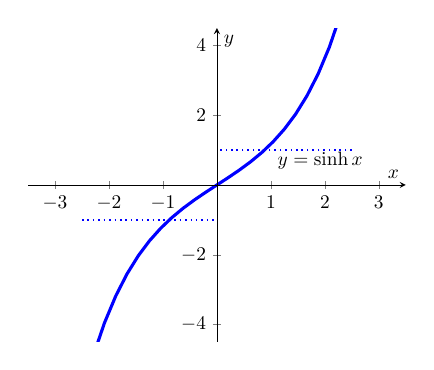
\begin{tikzpicture}[scale=0.7]
        \begin{axis}[
            xmin=-3.5, xmax=3.5,
            ymin=-4.5, ymax=4.5,
            axis lines=center,
            axis on top=true,
            domain=-2.5:2.5,
            ylabel=$y$,
            xlabel=$x$,]
            \addplot [mark=none,draw=blue,ultra thick] {sinh(\x)};
            \node [right, black] at (axis cs: 1,0.7) {$y = \sinh x$};
    
        %% Add the asymptotes
        \draw [blue, dotted, thick] (axis cs:-2.5,-1)-- (axis cs:0,-1);
        \draw [blue, dotted, thick] (axis cs:+2.5,+1)-- (axis cs:0,+1);
        \end{axis}
    \end{tikzpicture}
    \caption{Graph of F3} \label{fig:1.1}
    \end{figure}
Main characteristics of F3 is listed as below with proofs\cite{1}.

 \begin{itemize}
    \item F3 is an odd function.
    \begin{equation}
        \sinh x = -\sinh x
    \end{equation}
    
    \item F3 is one-to-one.
    \begin{equation}
        \frac{e^{m}-e^{-m}}{2} = \frac{e^{n}-e^{-n}}{2} \Leftrightarrow m = n
    \end{equation}
    
    \item F3 is onto.
    \begin{equation}
        \forall x \epsilon R, \exists y \epsilon R, \sinh x = y
    \end{equation}
        
    \item F3 is bijective function from \textbf{R} to \textbf{R}.
  \end{itemize}



\section{Requirements Specification}
\subsection{Purpose}
The purpose of this section is to give a detailed description of the requirements for the "calculator of F3"(CF3). It will illustrate the system constraints, assumptions, interfaces, functional and quality requirements of the system.

\subsection{Definitions, acronyms, and abbreviations}
    \begin{table}[htp]
    \centering
    \resizebox{\textwidth}{!}{%
    \begin{tabular}{|l|l|}
    \hline
    Term        & Definition                                                                                                                                                       \\ \hline
    CF3         & Calculator of F3, the name of the system.                                                                                                                        \\ \hline
    User        & Someone who interacts with CF3.                                                                                                                                  \\ \hline
    Stakeholder & Any person who has interaction with the system who is not a developer.                                                                                           \\ \hline
    DESC        & Description                                                                                                                                                      \\ \hline
    RAT         & Rational                                                                                                                                                         \\ \hline
    DEP         & Dependency                                                                                                                                                       \\ \hline
    TAG         & A unique, persistent identifier contained in a PLanguage statement\cite{2}                                                                                               \\ \hline
    GIST        & \begin{tabular}[c]{@{}l@{}}A short, simple description of the concept contained in a PLanguage\\ statement\cite{2}\end{tabular}                                          \\ \hline
    SCALE       & \begin{tabular}[c]{@{}l@{}}The scale of measure used by the requirement contained in a PLanguage\\ statement\cite{2}\end{tabular}                                        \\ \hline
    METER       & \begin{tabular}[c]{@{}l@{}}The process or device used to establish location on a SCALE contained in a PLanguage\\ statement \cite{2}\end{tabular}                                        \\ \hline
    MUST        & \begin{tabular}[c]{@{}l@{}}The minimum level required to avoid failure contained in a PLanguage\\ statement\cite{2}\end{tabular}                                         \\ \hline
    WISH        & \begin{tabular}[c]{@{}l@{}}A desirable level of achievement that may not be attainable through available\\ means contained in a PLanguage statement\cite{2}\end{tabular} \\ \hline
        \end{tabular}
        }
    \end{table}
\subsection{Constraints and Assumptions}
The CF3 application is constrained by the hardware and the maximum output that CF3 could calculate is 3.40282346638528860e+38 while the minimum output is -3.40282346638528860e+38.

One assumption about the CF3 application is that it will always be used to calculate numbers within constrained range which is (-	
89.41598623262829836363, 	
89.41598623262829836363).
\subsection{Interfaces Requirements}
The user interface should be Text-based User Interface(TUI). All interface requirements have high priority and they are normal difficulty.\\
\textbf{ID: IR1} \\
TITLE: Input a number \\
DESC: When program is executed, the user shall be able to see the instructions to input a number within 1s. \\
RAT: In order to input a number for calculation.\\
DEP: None\\
\textbf{ID: IR2} \\
TITLE: Show not-a-number error\\
DESC: When the input is not a valid number, the user shall be able to see an error message within 1s. \\
RAT: In order to make sure the input is a number.\\
DEP: IR1\\
\textbf{ID: IR3} \\
TITLE: Show out-of-bound error\\
DESC: When the input is not within the constrained range, the user shall be able to see an error message within 1s. \\
RAT: In order to make sure the output and calculation are within the CF3 application constraints.\\
DEP: IR1\\
\textbf{ID: IR4} \\
TITLE: Repeat inputs\\
DESC: When after user see error messages, the user shall be able to see instructions to input a number. \\
RAT: In order to make sure that user should input again after seeing error messages.\\
DEP: IR2, IR3\\
\textbf{ID: IR5} \\
TITLE: Output the result\\
DESC: When recieved a valid input, the user shall be able to see the calculated result. \\
RAT: In order to output the calculated result.\\
DEP: IR1\\
\subsection{Functional Requirements}
This section includes the requirements that specify all the fundamental actions of the software system.\\
\textbf{ID: FR1} \\
TITLE: Execute the application \\
DESC: When double click .exe file at a computer, the user shall be able to execute the application.\\
RAT: In order for a user to execute the application.\\
DEP: None\\
\textbf{ID: FR2} \\
TITLE: Input a number\\
DESC: When execute the application, the user shall be able to input a number. \\
RAT: In order to get the input for calculation.\\
DEP: FR1\\
\textbf{ID: FR3} \\
TITLE: Output a result\\
DESC: When a valid input is received, the user shall be able to get the calculated result within 1s.\\
RAT: In order to output the calculated result\\
DEP: FR2\\
\textbf{ID: FR4} \\
TITLE: Validate input\\
DESC: When an input is received, the CF3 application shall validate the input within 1s. \\
RAT: In order to make sure the input is valid.\\
DEP: FR2\\
\subsection{Performance Requirements}
\textbf{ID: QR1} \\
TITLE: ResponseTime\\
GIST: The fastness of the calculation\\
SCALE: The response time of the calculation\\
METER: Measurements obtained from 100 calculations\\
MUST: No more than 0.5 second 100 percent of the time\\
WISH: No more than 0.1 second 100 percent of the time\\
DESC: When an input is received, the CF3 application shall validate the input within 1s. \\
RAT: In order to make sure the input is valid.\\

\textbf{ID: QR2} \\
TITLE: Application testability\\
DESC: Test environments should be built for the application to allow testing of the applications different functions.\\
RAT: In order to test the application.\\

\textbf{ID: QR3} \\
TITLE: SystemReliability\\
GIST: The reliability of the system\\
SCALE: The reliability that the system gives the right result on a calculation\\
METER: Measurements obtained from 100 calculations during testing\\
MUST: 100 percent of the calculations\\

\subsection{Prioritization and Difficulty}
In order to get a view of how to divide the requirements into different iterations, following gives the priority and difficulty of the requirements.
    \begin {table}[!ht]
    \caption {Priority and Difficulty of the Requirements} \label{tab:title} 
    \centering
    \begin{tabular}{|c|c|c|} 
    \hline
    ID  & Priority & Difficulty  \\ 
    \hline
    IR1 & High     & Easy        \\ 
    \hline
    IR2 & High     & Easy        \\ 
    \hline
    IR3 & High     & Easy        \\ 
    \hline
    IR4 & Medium   & Normal      \\ 
    \hline
    IR5 & High     & Easy        \\ 
    \hline
    FR1 & Medium   & Easy        \\ 
    \hline
    FR2 & High     & Easy        \\ 
    \hline
    FR3 & High     & Easy        \\ 
    \hline
    FR4 & High     & Normal      \\ 
    \hline
    QR1 & High     & Normal      \\ 
    \hline
    QR2 & Medium   & Normal      \\ 
    \hline
    QR3 & Medium   & Normal      \\
    \hline
    \end{tabular}
    \end{table}
\end{normalsize}

\begin{thebibliography}{2}
\bibitem{1}
mathcentre, Universities of Loughborough \\
\textit{http://www.mathcentre.ac.uk/resources/workbooks/mathcentre/hyperbolicfunctions}

\bibitem{2}
Feldt R 
\textit{re_lecture5b_100914, unpublished}
\end{thebibliography}

\end{document}
